\section{Hardware details}
The hardware is implemented as three motherboards, onto each of which are mounted
three motor controller daughterboards. Each motherboard controls one
pair of motors. Screw connectors on the board connect the motors, potentiometers
and encoders; also the \isqc{} and power busses.

A circuit diagram and PCB layout for a single board can be found in the \emph{eagle} directory.

Each controller daughterboard has a unique \isqc{} address, which is set
as a parameter of the \emph{upload} script. 

\subsection{Procedure for updating the master firmware}
Ino (\verb+www.inotool.com+) must be installed to build the firmware, which
is then uploaded over the USB connection:
\begin{v}
cd rover/firmware/master
(edit code)
ino build
./upload
\end{v}
\subsection{Procedure for updating the slave firmware}
Ino (\verb+www.inotool.com+) must be installed to build the firmware, which
is then uploaded using a USBTiny ICSP programmer:
\begin{v}
cd rover/firmware/slave
(edit code)
\end{v}
and then either
\begin{v}
./blift
\end{v}
to build firmware for a lift/lift controller, or
\begin{v}
./bdrive
\end{v}
to build firmware for a drive/drive controller.
Then connect the ICSP to the controller and run
\begin{v}
./upload N
\end{v}
where $N$ is the controller number. It is possible to upload the software
to several different controllers without rebuilding it:
\begin{v}
./blift
./upload 3
./upload 6
./upload 9
./bdrive
./upload 1
./upload 2
./upload 4
./upload 5
./upload 7
./upload 8
\end{v}
is a typical scenario. Of course, you'll have to plug the programmer
onto the ICSP pins for the each board for each command.


\subsection{Pullup resistors}
Note that the \isqc{} internal pullup resistors are disabled on all
the microcontrollers. Therefore a pair of pullups of a suitable
value are added, pulling up to 3V. These are on a shield board mounted
onto the Arduino, along with an additional pullup for the OneWire bus
managing the temperature sensors.

\subsection{Controller assignments}
Figure~\ref{fig3} shows the controller/wheel assignments. For example,
the steer and drive wheel of controller 1 is wheel number 5, while
controller 3 controls the lift motors on wheels 5 and 6.

\subsection{Connections}
The following connections are used on the master:
\begin{itemize}
\item \textbf{USB} connection for control
\item \textbf{A4} for \isqc{} SDA line
\item \textbf{A5} for \isqc{} SCL line
\end{itemize}
The following connections are used on the DS(P) slaves:
\begin{itemize}
\item \textbf{M1+/M1-} for drive motor
\item \textbf{M2+/M2-} for steer motor
\item \textbf{ADC6} for steer potentiometer
\item \textbf{ADC7} for chassis potentiometer if present
\item \textbf{TX} for drive motor encoder channel A
\item \textbf{RX} for drive motor encoder channel B
\end{itemize}
The following connections are used on the LL slaves:
\begin{itemize}
\item \textbf{M1+/M1-} for lift motor 1
\item \textbf{M2+/M2-} for lift motor 2
\item \textbf{ADC6} for lift potentiometer 1
\item \textbf{ADC7} for lift potentiometer 2
\end{itemize}
The layout of a single board is shown in figure~\ref{boardfig}, while
the layout of all the boards inside the body of the rover is shown in
figure~\ref{internalwiring}.

\begin{figure}[ht]
\center
\includegraphics[width=3in]{boardDrawing.pdf}
\caption{Board connections}
\label{boardfig}
\end{figure}

\begin{figure}[ht]
\center
\includegraphics[width=5in]{internalWiring.pdf}
\caption{Internal layout of the main rover compartment}
\label{internalwiring}
\end{figure}

\clearpage
\subsubsection{Connection labelling}
Wires running to the motors --- both sensor and motor control wires ---
are marked using coloured rings of insulation.
Figures \ref{senscols} and \ref{motorcols} show the schemata used.
Note that in both diagrams, the proximal (motor controller board) end is shown to the
right.

\begin{figure}[ht]
\center
\includegraphics[width=5in]{sensors1.pdf}
\caption{Sensor wire labelling scheme}
\label{senscols}
\end{figure}


\begin{figure}[ht]
\center
\includegraphics[width=5in]{motors1.pdf}
\caption{Motor wire labelling scheme}
\label{motorcols}
\end{figure}

Other colours:
\begin{itemize}
\item \isqc{} bus : blue and white twisted pair --- the white line is the SDA, the
blue line is SCL.
\item Power bus : black and red twisted pair --- red is +12V, black is ground
\item Power input : brown is +12V, green/yellow is ground
\item OneWire bus : orange and orange/white twisted pair --- orange is ground,
orange/white is data
\item Chassis lines: red is +5V, black is ground, yellow is data. There's
no ID marking; the line can be clearly traced to its potentiometer by eye.
\end{itemize}
\clearpage
\subsection{Remote control connections}
The remote control is connected to the master Arduino Uno as shown in
figure~\ref{fig:remo}.
\begin{figure}[ht]
\center
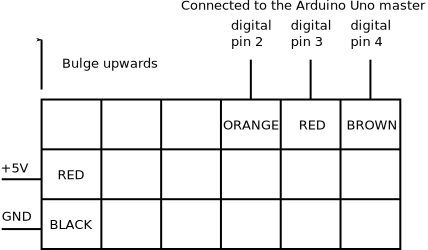
\includegraphics[width=4in]{remote.pdf}
\caption{Servo receiver connections}
\label{fig:remo}
\end{figure}


